\documentclass[12pt]{article}
\usepackage[czech]{babel}
\usepackage{natbib}
\usepackage{url}
\usepackage[utf8x]{inputenc}
\usepackage{amsmath}
\usepackage{graphicx}
\graphicspath{{images/}}
\usepackage{parskip}
\usepackage{fancyhdr}
\usepackage{vmargin}
\setmarginsrb{3 cm}{2.5 cm}{3 cm}{2.5 cm}{1 cm}{1.5 cm}{1 cm}{1.5 cm}
\usepackage{fancyhdr}
\usepackage{caption}
\usepackage{array}
\newcolumntype{?}[1]{!{\vrule width #1}}
\usepackage{hyperref}
\usepackage{unicode-math}
\hypersetup{
    colorlinks=true,
    linkcolor=red,
    filecolor=red,
    urlcolor=blue,
    citecolor=red,
    linktoc=none
    }


\makeatletter
\let\thetitle\@title


\makeatother

\pagestyle{fancy}
\fancyhf{}
\rhead{\theauthor}
\lhead{\thetitle}
\cfoot{\thepage}

%%%%%%%%%%%%%%%%%%%%%%%%%%%%%%%%%%%%%%%%%%%%%%%%%%%%%%%%%%%%%%%%%%%%%%%%%%%%%%%%%%%%%%%%%
\begin{document}
\afterpage{\cfoot{\thepage }}

\section{Odd-even merge sort}
 Odd-even merge sort je řadicí algoritmus, který pracuje na principu spojování dvou již seřazených posloupností. Schéma je složeno z bloků:
 \begin{itemize}
     \item 1x1 -- vstupem jsou dvě seřazené posloupnosti o jednotkové velikosti a výstupem je seřazení těchto dvou hodnot.
     \item 2x2 -- vstupem jsou dvě seřazené posloupnosti o velikost dva a výstupem jsou čtyři seřazené hodnoty.
     \item 4x4 -- ...
 \end{itemize}
 
Jedná se o algoritmus typicky používaný v HW, protože každý blok je ve výsledku složen z 1x1 bloků, které představují velmi jednoduché procesory -- umí přijmout, porovnat a umístit na výstup dvě hodnoty. Jelikož jsou procesory napevno zapojeny, je napevno dána i velikost řazené posloupnosti (mocnina dvou). Pokud je řazených hodnot méně, lze je doplnit "paddingem". Při fixní velikosti \(n\) řazené posloupnosti lze vypočítat, že poslední vrstva obsahuje nejvetší blok \(n/2\) x \(n/2\). Tento blok předchází dvojnásobný počet bloků o velikosti \(n/4\) x \(n/4\) atd. až do velikosti bloku 1x1.

\subsection{Analýza časové složitosti}
Jak již bylo zmíněno a jak je také vidět v obrázku \ref{diagram}, velikost bloku poslední vrstvy je \(n/2\) x \(n/2\). Když si velikost vstupu zapíšeme jako \(n = 2^m\), tak číslo \(m\) lze chápat jako index poslední vrstvy, číslo \(m-1\) index předposlední vrstvy, ..., až \(1\) je index první vrstvy -- bloky 1x1. Z tohoto je jasné, že časová složitost je suma časových složitostí vrstev \(1\) až \(m\). Jelikož jsou bloky v každé vrstvě zapojeny paralelně, tak se tato suma zjednoduší na sumu časových složitostí bloků 1x1, ..., \(n/2\) x \(n/2\). V obrázku \ref{diagram} lze vidět, že každý blok \(n\) x \(n\) (vyjma 1x1) je tvořen dvěma paralelně zapojenými bloky \(n/2\) x \(n/2\) a za nimi vrstvou bloků 1x1. Z tohoto vyplývá, že každá vrstva má složitost \(t_m = t_{m-1} + 1\). Jelikož \(t_1 = 1\) lze celkovou složistot tohoto algorimu vyjádřit jako:

\[\sum\limits_{i=1}^m i = \frac{1}{2}m(m+1)\]

Když víme, že:

\[m=\log_2 n\]

pak lze předchozí výraz přepsat na závislost vůči \(n\) takto:

\[\frac{1}{2}\log_2 n(\log_2 n+1)\]
 
Po odstranění multiplikativních a aditivních konstant:

\[\log n \log n\in O(\log^2 n)\] 

\subsection{Analýza prostorové složitosti}
Zde opět využijeme indexovaní vrstev, tzn. \(m\) značí poslední vrstvu, \(m-1\) předposlední atd. Počet procesorů každé vrstvy (kromě první) je roven počtu procesorů předchozí vrstvy + přidané bloky 1x1 (procesory). Je tedy nutné obecně vyjádřit počet přidaných bloků 1x1 pro blok \(x\) x \(x\), vučí bloku \((x-1)\) x \((x-1)\). Uvažujme \(j\)-tou vrstvu, která je složena z bloků \(\frac{2^j}{2}\) x \(\frac{2^j}{2}\), kde \(2^j\) značí počet vstupů bloku \(j\)-té vrstvy. Víme, že nejmenší a největší prvek v každém bloku je přímo napojen na výstup. Zbylé prvky jsou rozděleny do dvojic a každá je porovnána jedním 1x1 blokem. Z toho nám vychází, že počet přidaných bloků 1x1 pro blok \(\frac{2^j}{2}\) x \(\frac{2^j}{2}\), které tvoří \(j\)-tou vrstvu je:

\[\frac{2^j - 2}{2}\]

Ovšem bloků \(\frac{2^j}{2}\) x \(\frac{2^j}{2}\) v \(j\)-té vrstvě může být více. Počet těchto bloků v dané vrsvě pro vstup o velikosti \(n\) je:

\[\frac{n}{2^j}\]

Nyní jsme schopni vyjádřit přírůstek 1x1 bloků vrstvy \(j\) oproti vrstvě \(j-1\):

\[\frac{n}{2^j}\frac{2^j - 2}{2}\]

Tento výraz je konstruován tak, aby pro \(j=1\) byl přírůstek roven 0. Tzn. první vrstva nemá žádný přírůstek, proto je nutné nutně explicitně přidat \(n/2\) 1x1 bloků, které jsou na začátku každé vrstvy, viz. obrázek \ref{diagram}. Nyní už jsme schopni sepsat výraz vyjadřující počet procesorů pro vstup o velikosti \(n\):

\[(\frac{n}{2}+\frac{n}{2^1}\frac{2^1 - 2}{2}) + 
  (\frac{n}{2}+\frac{n}{2^1}\frac{2^1 - 2}{2} + \frac{n}{2^2}\frac{2^2 - 2}{2}) +
   ... + 
  (\frac{n}{2}+\frac{n}{2^1}\frac{2^1 - 2}{2} + \frac{n}{2^2}\frac{2^2 - 2}{2} + ... + \frac{n}{2^m}\frac{2^m - 2}{2})\]

Tento výraz můžeme upravit na:
\[(\frac{n}{2^1}\frac{2^1 - 2}{2}) + 
  (\frac{n}{2^1}\frac{2^1 - 2}{2} + \frac{n}{2^2}\frac{2^2 - 2}{2}) +
   ... + 
  (\frac{n}{2^1}\frac{2^1 - 2}{2} + \frac{n}{2^2}\frac{2^2 - 2}{2} + ... + \frac{n}{2^m}\frac{2^m - 2}{2}) + m\frac{n}{2}\]

Závorky můžeme nyní přepsat do tvaru sum:
\[\sum\limits_{i=1}^m (\sum\limits_{j=1}^i (\frac{n}{2^j}\frac{2^j-2}{2}))+ m\frac{n}{2}\]

Nyní dosadíme za \(m\):
\[\sum\limits_{i=1}^{\log_2 n} (\sum\limits_{j=1}^i (\frac{n}{2^j}\frac{2^j-2}{2}))+ \log_2 n\frac{n}{2}\]

Pomocí WolframAlpha\footnote{WolframAlpha -- matematický software \href{https://www.wolframalpha.com}{https://www.wolframalpha.com}.} převedeme součet řady na výraz bez sum:

\[n + \frac{n \log^2 n}{4 \log^2 2} - \frac{n \log 8 \log n}{4 \log^2 2} + \frac{n \log n}{2 \log 2} - 1\]

Odstraníme aditivní a multiplikativní konstanty:
\[n + n \log^2 n - n\log n + n \log n\]

Ponecháme pouze nejdominantnější výraz:
\[n \log^2 n \in O(n \log^2 n) \] 

\subsection{Analýza ceny}
Cenu vypočítáme z časové a prostorové složitosti následovně:

\[n \log^2 n \log^2 n = n \log^4 n \in O(n \log^4 n)\]

Je jasné, že cena \textbf{není optimální}. To lze poznat už z obrázku \ref{diagram}, protože každý "worker" procesor učiní pouze jediné porovnání a zbytek času je neaktivní.

\section{Implementace}
Jelikož se jedná o HW řadící algoritmus bylo nutné simulovat procesory pomocí procesů. Toto ovšem není ideální, protože všechny určitě nepoběží zároveň, tak jak by tomu bylo při HW obvodu. Fyzické propojení procesorů je nahrazeno zasíláním asynchronních zpráv mezi procesy. 

Schéma zapojení/komunikace je znázorněno na obrázku \ref{diagram}. Čísla značí rank procesů a šipky značí směr komunikace. Každá šipka znázorňuje přenos jediné hodnoty. Propojení jsou napevno specifikována poli \texttt{min\_out} a \texttt{max\_out}, která jsou přístupná všem procesům a ty si z nich vybírají informace, kam výsledky poslat na základě svého ranku (použitého jako index). Odesílání minimální/maximální hodnoty je znázorněno šipkou z pravého horního/dolního rohu procesu.

Oproti HW zapojení SW implementace obsahuje navíc proces s rank 0 (master), který zajišťuje načtení hodnot a jejich rozeslání první vrstvě procesů a na konci sesbírání a vypsaní hodnot. Zvolil jsem tento přístup, protože umožňuje čistější oddělení implementace a nenastane případ, že by se procesy zasekávaly na zámcích souborů.

Každý worker proces čeká na dvě příchozí asynchronní zprávy. Jelikož je zapojení pevně dáno, nemůže se stát, že dostane jiný počet zpráv nebo od nesprávného procesu. Po obdržení zpráv jsou hodnoty porovnány a opět asnychronně poslány dále.

\section{Závěr}
Odd-even merge sort pracuje s pevným počtem procesorů, který je dán velikostí vstupu. Jelikož ze zadání byla velikost vstupu zafixována na 8, tak nemá implementace žádnou proměnlivou strukturu. Vyhodocení pro různé nastavení tudíž nedává smysl. 

Rovněž nemá smysl měřit výkonost algoritmu, protože se jedná o SW simulaci HW obvodu, jehož jedinou funkční části by mělo být porovnávání hodnot. Nicméně režie na vytváření, přepínání a komunikaci mezi procesy velmi převýší čas ztrávený porovnáváním hodnot (troufám si odhadovat, že 99,99 \% připadne režii procesů). 

Výhodou SW simulace by mohl být fakt, že stačí použít pouze \(n/2\) procesů (první vrstva), protože právě takové množství jich může maximálně pracovat současně. Další prpojení by pak byla závislá na fázi v jaké se výpočet nachází. Toto je samozřejmě možné vytvořit i v HW obvodu, ale procesory už by se musely zesložit, což nemusí být žádoucí (CPU je pro tento problém dostatečně generické).

\hspace{-2cm}
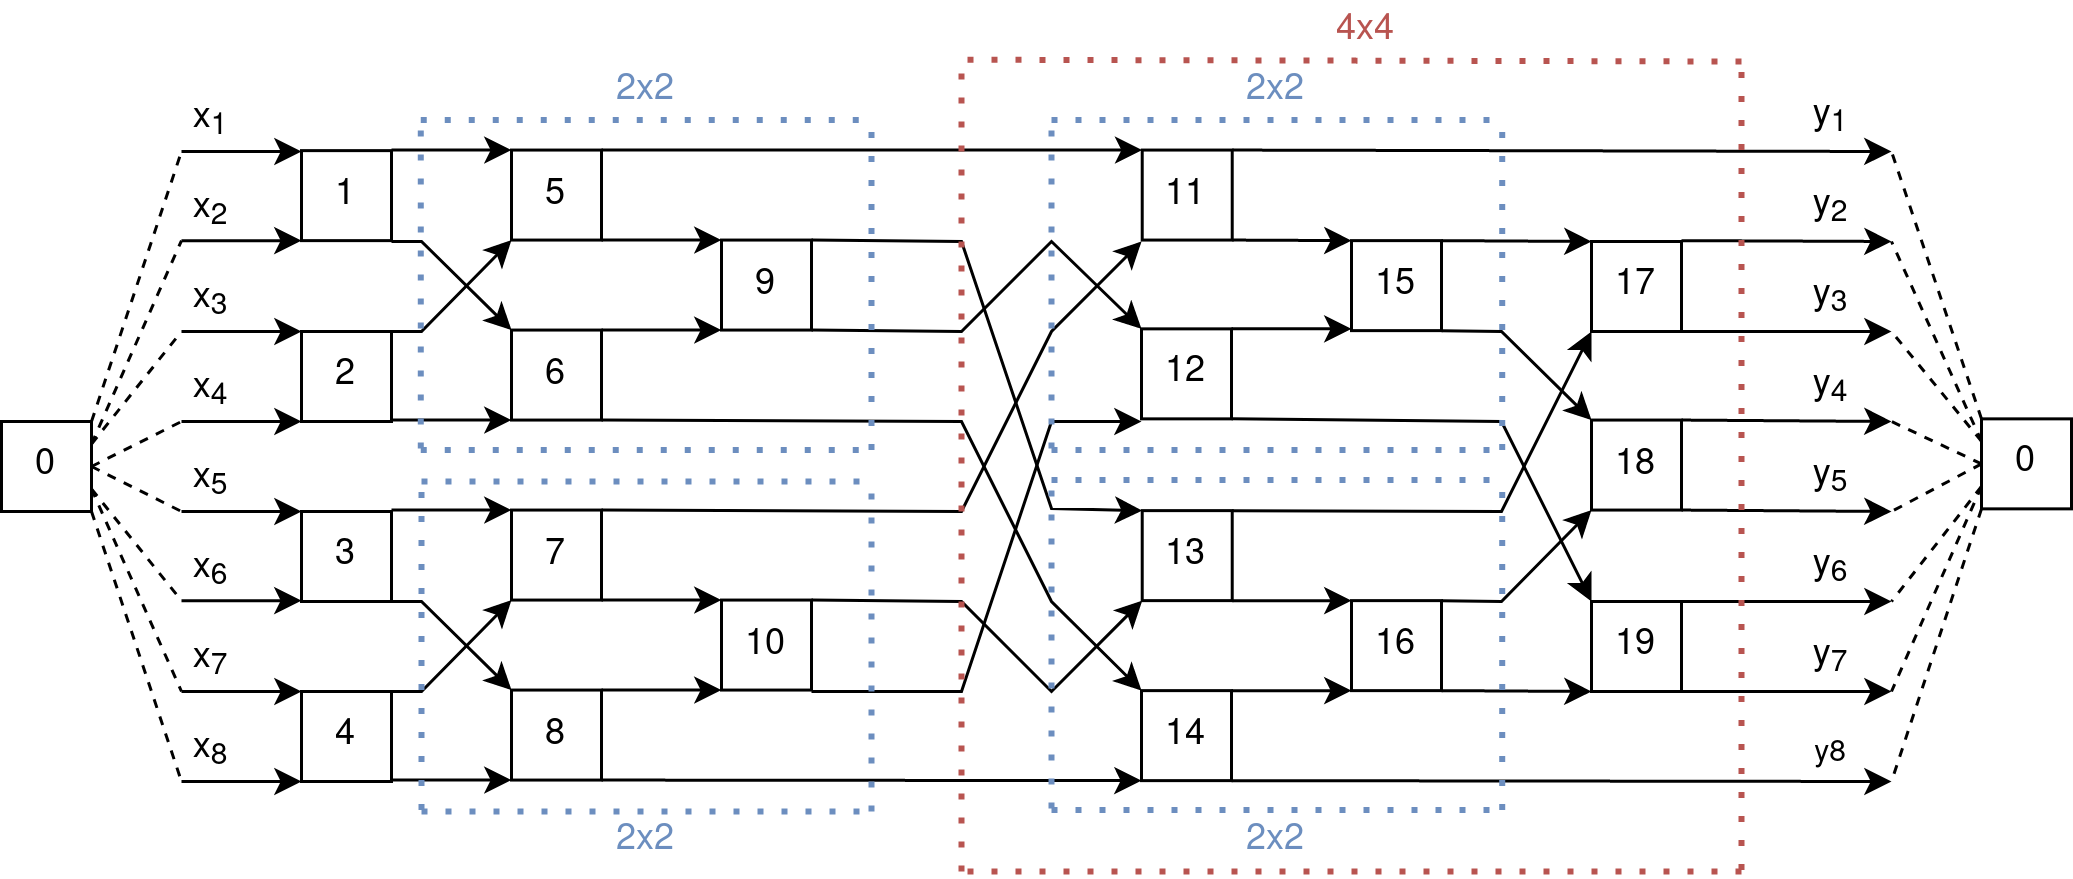
\includegraphics[width=0.9\paperwidth]{4x4-diagram.png}
\captionof{figure}{Diagram komunikace procesů pro řazení 8 hodnot, při použití Odd-even merge sort. Procesor 0 značí tzv. "master" proces a procesy 1-19 tzv. "worker" procesy.}
\label{diagram}

\end{document}
